\documentclass[journal, a4paper]{IEEEtran}
\IEEEoverridecommandlockouts
\usepackage{graphicx}
\usepackage{booktabs}
\usepackage{times}
\usepackage{amsmath}
\usepackage[tableposition=top]{caption}
\usepackage[section]{placeins}
\usepackage{float}
\usepackage{cite}
\usepackage{hyperref}
\hypersetup{pdfauthor={Muhamad Kemal Faza, Muchammad Yuda Tri Ananda, Muhammad Akmal Fazli Riyadi, Henri Tantyoko}, pdfsubject={GEMASTIK XVIII Data Mining}, colorlinks=true, citecolor=blue, urlcolor=blue}
\graphicspath{{./}}
\setlength{\parindent}{1em}
\setlength{\parskip}{0.5ex}

\renewcommand{\figurename}{Gambar}
\renewcommand{\tablename}{Tabel}

\begin{document}

\twocolumn[
  \begin{@twocolumnfalse}
    \begin{center}
      \vspace{1.5em}
      {\sffamily\bfseries\huge PanganFlow.ID: Penambangan Pola Surplus-Defisit dan Rekomendasi
      Redistribusi Beras Antarprovinsi Berbasis Disparitas Harga,
      Produksi, dan Konsumsi \par}
      \vspace{1.2em}
      
      {\sffamily\bfseries\large Muhamad Kemal Faza$^{1}$, Muchammad Yuda Tri Ananda$^{2}$, Muhammad Akmal Fazli Riyadi$^{3}$, Henri Tantyoko$^{4}$ \par}
      \vspace{0.8em}
      
      {\small $^{1}$Fakultas Sains dan Matematika, Universitas Diponegoro, Semarang, 50275, email: kemalfaza26@students.undip.ac.id \\
      $^{2}$Fakultas Sains dan Matematika, Universitas Diponegoro, Semarang, 50275, email: myudak@students.undip.ac.id \\
      $^{3}$Fakultas Sains dan Matematika, Universitas Diponegoro, Semarang, 50275, email: akmalfazli27@students.undip.ac.id \\
      $^{4}$Fakultas Sains dan Matematika, Universitas Diponegoro, Semarang, 50275, email: henritantyoko@lecturer.undip.ac.id \par}
      \vspace{0.5em}
      
      {\small\textit{Corresponding Author}: Muhamad Kemal Faza \par}
    \end{center}
    \vspace{1.5em}
    
    \noindent\textbf{\sffamily INTISARI} --- Ketahanan pangan nasional tidak hanya ditentukan oleh kecukupan stok secara agregat, tetapi juga dipengaruhi disparitas pasokan dan aksesibilitas antarwilayah. Sebagai kontribusi nyata dalam bidang peningkatan Teknologi Informasi dan Komunikasi (TIK) menuju kemandirian pangan bangsa, penelitian ini mengembangkan PanganFlow.ID. Sistem penambangan data (\textit{data mining}) spatio-temporal terpadu ini dirancang untuk mendeteksi tingkat kerentanan pasokan beras tingkat daerah dan menyusun prioritas aliran redistribusi pangan antarprovinsi. Dataset panel yang dikaji mencakup 1.904 observasi provinsi-bulan untuk 38 provinsi pada periode Januari 2021 hingga Juni 2025, yang diintegrasikan dari portal resmi Badan Pangan Nasional (Bapanas), Badan Pusat Statistik (BPS), dan Bank Indonesia. Metode yang diimplementasikan meliputi deteksi anomali harga berbasis Isolation Forest, estimasi proxy neraca surplus-defisit, pemodelan prioritas dengan Random Forest, pemetaan tipologi wilayah melalui K-Means clustering, serta perancangan \textit{graph-based redistribution scoring}. PanganFlow.ID berhasil mengidentifikasi wilayah rentan prioritas secara objektif dan menyajikan rekomendasi pasangan provinsi surplus-defisit yang optimal sebagai bahan tinjauan kebijakan distribusi nasional yang presisi.
    
    \vspace{0.8em}
    \noindent\textbf{\sffamily KATA KUNCI} --- Penambangan Data, Beras, Ketahanan Pangan, Kemandirian Bangsa, Aliran Redistribusi, Deteksi Anomali.
    \vspace{2.0em}
  \end{@twocolumnfalse}
]


\section{Pendahuluan}
Kemandirian bangsa yang kokoh berakar pada ketahanan sektor strategisnya, salah satunya adalah pangan. Indonesia secara nasional memiliki kecukupan produksi beras, namun disparitas harga antarprovinsi menunjukkan adanya ketidakseimbangan distribusi spasial. Data Badan Pangan Nasional (Bapanas) periode 2021--2025 menunjukkan harga eceran beras medium di Papua Pegunungan menembus Rp25.500/kg, hampir dua kali lipat dibanding Jawa Timur yang hanya Rp12.742/kg. Selisih ekstrem ini tidak semata dipicu oleh kendala transportasi logistik, melainkan merefleksikan ketimpangan struktural jangka panjang antara wilayah produsen (surplus) dan konsumen (defisit).

Dari 38 provinsi di Indonesia, hanya 14 provinsi yang mencatat surplus produksi beras (terkonsentrasi di Pulau Jawa dan Sulawesi Selatan), sedangkan 24 provinsi lainnya secara konsisten mengalami defisit pasokan lokal. Region Maluku-Papua merupakan wilayah yang paling rentan; seluruh provinsi di wilayah tersebut mengalami defisit produksi struktural dengan tingkat harga eceran melampaui median nasional. Kondisi geografis kepulauan Indonesia menuntut adanya pendekatan Teknologi Informasi dan Komunikasi (TIK) yang cerdas dan prediktif. Pemanfaatan metodologi \textit{data mining} spatio-temporal berbasis multi-sumber menjadi langkah inovatif guna menambang pola distribusi serta memitigasi disparitas pasokan secara presisi demi mendukung tercapainya kemandirian pangan nasional.

Fokus penelitian ini adalah mengembangkan sistem \textit{data mining} PanganFlow.ID untuk memecahkan tiga rumusan masalah utama: (1) provinsi mana yang mengalami tekanan pasokan dan gejolak harga pangan paling kritis, (2) wilayah mana yang memiliki potensi surplus terbesar untuk menyokong kebutuhan daerah lain, serta (3) pasangan asal-tujuan (\textit{flow}) antardaerah mana yang menjadi prioritas utama untuk intervensi redistribusi. Adapun batasan masalah dalam penelitian ini didefinisikan sebagai berikut: (1) komoditas dibatasi pada Beras Medium untuk menjaga konsistensi data produksi BPS dan harga eceran Bapanas; (2) neraca surplus-defisit dihitung berdasarkan estimasi kebutuhan tahunan kolektif (\textit{proxy} struktural), bukan mencerminkan stok fisik harian di gudang; dan (3) rekomendasi aliran redistribusi diposisikan sebagai acuan prioritas tinjauan kebijakan pemerintah, bukan sebagai perintah logistik operasional final.



\section{Kajian Terkait}
Prediksi harga pangan dan deteksi anomali telah banyak diteliti dalam literatur data mining.
Sediyono dan Hartomo (2025) mengembangkan integrated framework untuk multi-commodity
agricultural price forecasting dan anomaly detection menggunakan Transformer-based models
dengan attention-boosted LSTM-VAE \cite{1}. Pendekatan serupa dengan semantic dan temporal fusion
untuk commodity price shock early warning juga telah dieksplorasi menggunakan agentic
generative AI \cite{2}.

Di Indonesia, beberapa studi membandingkan model LSTM, Random Forest, dan SVR untuk
prediksi harga beras di Sumatera Selatan, dengan hasil bahwa LSTM unggul untuk data
time-series \cite{3}. Di Jawa Barat, perbandingan ARIMA, Regresi Linear, Random Forest, dan
LSTM untuk harga beras medium harian menemukan bahwa ensemble methods memberikan
keseimbangan akurasi dan interpretabilitas \cite{4}. Pengaruh cuaca terhadap harga beras di
Jawa Timur juga telah dimodelkan menggunakan LSTM, menunjukkan bahwa fitur meteorologis
meningkatkan akurasi prediksi \cite{5}.

Dari sisi ensemble learning, stacking untuk prediksi harga beras nasional menunjukkan
bahwa kombinasi model dapat mengungguli model tunggal \cite{6}. Sementara itu, deep learning
hybrid untuk forecasting produksi beras di Indonesia memberikan perspektif berbeda karena
berfokus pada ketersediaan pasokan, bukan harga \cite{7}. Di tingkat distribusi, analisis
spasial-temporal untuk logistik rantai dingin produk pertanian menunjukkan pentingnya
faktor geografis dalam perencanaan distribusi pangan \cite{8}. Penelitian crop redistribution
secara global menunjukkan bahwa optimasi spasial dapat meningkatkan produksi sambil
mengurangi tekanan sumber daya \cite{9}. Model spatial equilibrium untuk perdagangan
antarwilayah pada distribusi gandum menunjukkan bahwa price signal dan biaya transportasi
adalah faktor kunci dalam aliran komoditas \cite{10}.

Kesenjangan utama dalam literatur yang ada adalah: (1) sebagian besar studi fokus pada
prediksi harga titik (point forecasting) di satu provinsi, bukan ranking prioritas
multi-provinsi; (2) belum ada penelitian yang mengintegrasikan sinyal harga, neraca
produksi-konsumsi, dan jarak geografis ke dalam satu sistem rekomendasi aliran
redistribusi untuk pangan Indonesia; (3) belum ada studi data mining di Indonesia yang
membingkai masalah pangan sebagai ranking prioritas intervensi. PanganFlow.ID mengisi
kesenjangan ini dengan menggabungkan anomaly detection, surplus-deficit proxy estimation,
Random Forest ranking, dan graph-based redistribution scoring menjadi pipeline terpadu.



\section{Dataset dan Formulasi Masalah}
Dataset final berbentuk panel provinsi-bulan-komoditas sebanyak 1.904 baris, mencakup 38 provinsi dan periode 1 Januari 2021 sampai 1 Juni 2025. Komoditas dibatasi pada Beras Medium agar perhitungan surplus-defisit konsisten dengan data produksi beras Badan Pusat Statistik (BPS) \cite{16} dan konsumsi beras per kapita tahunan \cite{17}. Harga pangan eceran bersumber dari Badan Pangan Nasional (Bapanas) \cite{15}, sedangkan referensi pelengkap dihimpun dari Pusat Informasi Harga Pangan Strategis (PIHPS) Bank Indonesia \cite{14}.

\begin{table}[H]
  \scriptsize
  \caption{Status sumber data resmi dan snapshot.}
  \label{tab:source_status}
  \begin{tabular}{lrr}
    \toprule
    source & status & rows \\
    \midrule
    BI PIHPS Province Reference & downloaded & 35 \\
    BI PIHPS Commodity Reference & downloaded & 31 \\
    BI PIHPS Daily Price Attempt (Medium I) & downloaded & 0 \\
    BI PIHPS Daily Price Attempt (Medium II) & downloaded & 0 \\
    BI PIHPS Manual Snapshot & not\_provided & 0 \\
    Bapanas Monthly Consumer Price & loaded & 1904 \\
    \bottomrule
  \end{tabular}
\end{table}

Kebutuhan beras daerah diproksikan sebagai jumlah populasi dikalikan konsumsi beras per kapita tahunan (81,23 kg/tahun) \cite{17}. \textit{Surplus proxy} dihitung sebagai total produksi beras tahunan \cite{16} dikurangi total kebutuhan tahunan. Mengingat ketiadaan data stok fisik riil antargudang bulanan yang bersifat publik dan \textit{open-access}, nilai neraca ini diperlakukan sebagai \textit{proxy} struktural spatio-temporal.



\section{Metodologi}
\textit{Pipeline} PanganFlow.ID dirancang dalam enam tahapan sistematis. Pertama, data harga beras medium konsumen dari Bapanas \cite{15} ditransformasikan menjadi serangkaian fitur dinamis, meliputi: selisih (\textit{gap}) terhadap median nasional, laju perubahan harga 1 dan 3 bulan, \textit{rolling mean} 3 bulan, \textit{rolling standard deviation} 6 bulan, serta \textit{z-score} historis 6 bulan. Kedua, data produksi beras BPS \cite{16} dikombinasikan dengan estimasi konsumsi per kapita \cite{17} untuk menghitung \textit{surplus/deficit proxy score} yang dinormalisasi menggunakan metode min-max. Ketiga, algoritme \textit{Isolation Forest} \cite{12} dengan tingkat kontaminasi (\textit{contamination}) sebesar 18\% diimplementasikan untuk mendeteksi sinyal anomali lonjakan harga lokal.

Keempat, regresi \textit{Random Forest} \cite{11} dengan konfigurasi hiperparameter optimal (\texttt{n\_estimators=260}, \texttt{min\_samples\_leaf=3}, \texttt{random\_state=42}) digunakan untuk mempelajari pola prioritas wilayah sasaran intervensi pada bulan berikutnya menggunakan \textit{temporal split} (15\% data akhir sebagai \textit{holdout set} pengujian). Kelima, metode \textit{K-Means clustering} \cite{13} (\texttt{k=4}, \texttt{n\_init=20}) dengan reduksi dimensi PCA 2 komponen digunakan untuk memetakan tipologi spasial ketahanan beras tiap provinsi. Keenam, hubungan \textit{flow} logistik antarpasangan provinsi surplus-defisit dianalisis secara grafis berdasarkan jarak geografis (\textit{Haversine}) dan kombinasi sinyal ekonomi melalui formula prioritas berikut:

\begin{equation}
\begin{aligned}
\text{priority\_score} =\ & 0,31 \times \text{price\_gap} + 0,27 \times \text{deficit} \\
& + 0,23 \times \text{surplus} + 0,14 \times \text{model} \\
& + 0,10 \times \text{anomaly} - 0,15 \times \text{distance}
\end{aligned}
\end{equation}

Model hibrida akhir menggabungkan \textit{weighted priority index} linear dengan skor prediksi non-linear dari \textit{Random Forest} melalui perpaduan pembobotan berikut:
\begin{equation}
\text{score} = 0,72 \times \text{weighted\_index} + 0,28 \times \text{rf\_prediction\_norm}
\end{equation}

Lima baseline digunakan sebagai pembanding:
\begin{enumerate}
    \item Ranking acak sebagai batas bawah.
    \item \textit{Price-gap ranking} untuk efek disparitas harga.
    \item \textit{Deficit ranking} untuk efek neraca.
    \item \textit{Weighted priority index} transparan.
    \item \textit{Random Forest ranker} dengan split temporal.
\end{enumerate}



\section{Eksperimen dan Hasil}
Untuk mengevaluasi performa model, lima \textit{baseline} digunakan sebagai pembanding: \textit{random ranking}, \textit{price-gap baseline}, \textit{deficit baseline}, \textit{weighted priority index}, dan model hibrida PanganFlow. Metrik utama yang digunakan adalah NDCG@K yang mengukur kualitas peringkat provinsi prioritas. Metrik Precision@K dan Recall@K melengkapi evaluasi untuk mengukur tingkat akurasi operasional pada peringkat teratas.

Tabel \ref{tab:metrics} dan Gambar \ref{fig:model_comparison} memaparkan bahwa model hibrida PanganFlow mencapai NDCG@K sebesar 0,937, mengungguli \textit{weighted index} (0,929) serta seluruh \textit{baseline} lainnya. Meskipun peningkatan (\textit{lift}) terhadap \textit{weighted index} relatif kecil (0,9\%), model regresi \textit{Random Forest} berhasil menangkap pola interaksi non-linear antarlapisan fitur yang tidak terdeteksi oleh indeks pembobotan linear sederhana.

Tabel \ref{tab:ablation} menyajikan hasil studi ablasi (\textit{ablation study}) terhadap kontribusi masing-masing kelompok fitur. Fitur neraca pangan (\textit{balance}) terbukti menjadi kontributor terbesar bagi performa model; ketiadaan fitur ini menurunkan NDCG@K dari 0,905 menjadi 0,880. Sebaliknya, fitur spasial memberikan kontribusi marginal terkecil karena efek kedekatan geografis sebagian besar telah direpresentasikan oleh pengelompokan wilayah (\textit{region grouping}).

Gambar \ref{fig:feature_importance} dan Gambar \ref{fig:shap_summary} mengonfirmasi dominasi fitur harga dan neraca pangan dalam prediksi model, dengan variabel \texttt{surplus\_proxy\_ton} dan \texttt{price\_gap\_score} menempati peringkat teratas dalam skor kepentingan fitur (\textit{feature importance}). Analisis \textit{error} spasial (Tabel \ref{tab:error}) menunjukkan bahwa wilayah Maluku-Papua mencatat tingkat kesalahan prediksi tertinggi, merefleksikan volatilitas data yang dinamis di Indonesia bagian timur.

\begin{table}[H]
  \footnotesize
  \caption{Hasil evaluasi peringkat provinsi prioritas.}
  \label{tab:metrics}
  \begin{tabular}{lrrr}
    \toprule
    Model & NDCG@K & Precision@K & Recall@K \\
    \midrule
    Random ranking & 0,294 & 0,300 & 0,300 \\
    Price-gap baseline & 0,826 & 0,750 & 0,750 \\
    Deficit baseline & 0,852 & 0,800 & 0,800 \\
    Weighted index & 0,929 & 0,900 & 0,900 \\
    PanganFlow & 0,937 & 0,910 & 0,910 \\
    \bottomrule
  \end{tabular}
\end{table}

\begin{figure}[H]
  \centering
  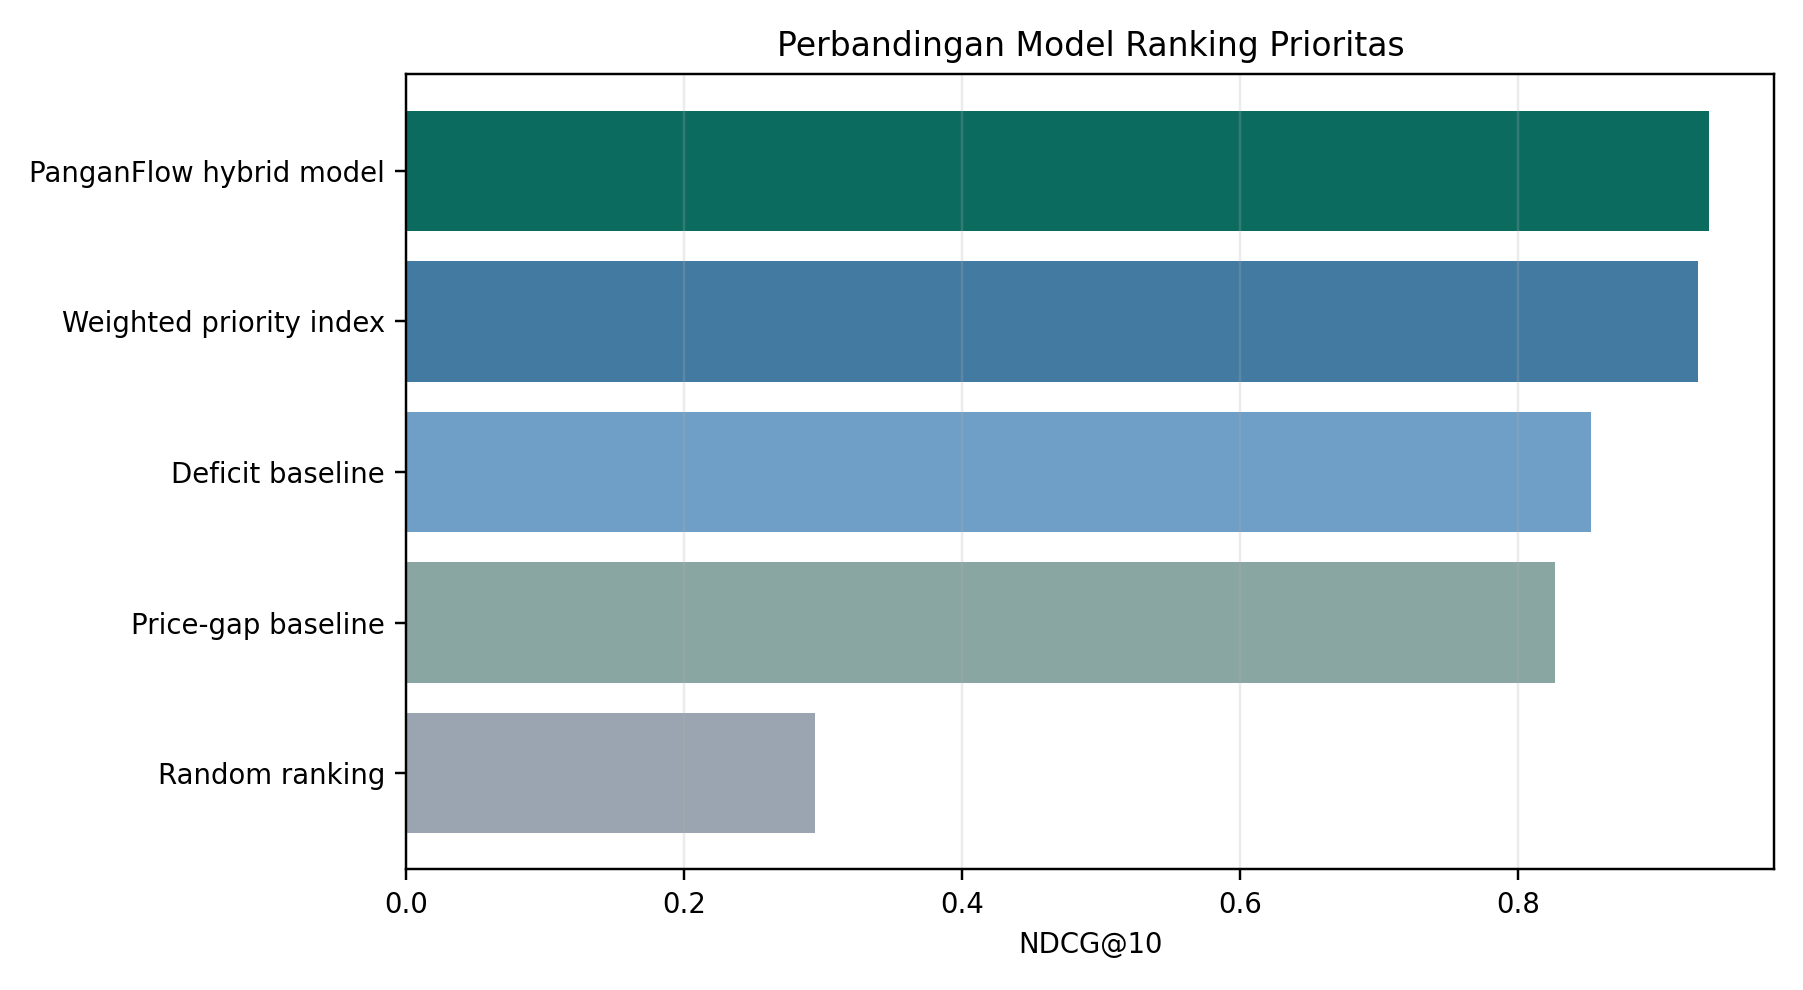
\includegraphics[width=0.48\columnwidth]{figures/model_comparison.png}
  \caption{Perbandingan NDCG@K antar model.}
  \label{fig:model_comparison}
\end{figure}

\begin{table}[H]
  \footnotesize
  \caption{Studi ablasi kontribusi keluarga fitur.}
  \label{tab:ablation}
  \begin{tabular}{lrrr}
    \toprule
    Konfigurasi Fitur & NDCG@K & Precision@K & Recall@K \\
    \midrule
    Tanpa spasial & 0,912 & 0,870 & 0,870 \\
    Semua fitur & 0,905 & 0,860 & 0,860 \\
    Tanpa fitur harga & 0,897 & 0,860 & 0,860 \\
    Tanpa fitur neraca & 0,880 & 0,830 & 0,830 \\
    \bottomrule
  \end{tabular}
\end{table}

\begin{figure}[H]
  \centering
  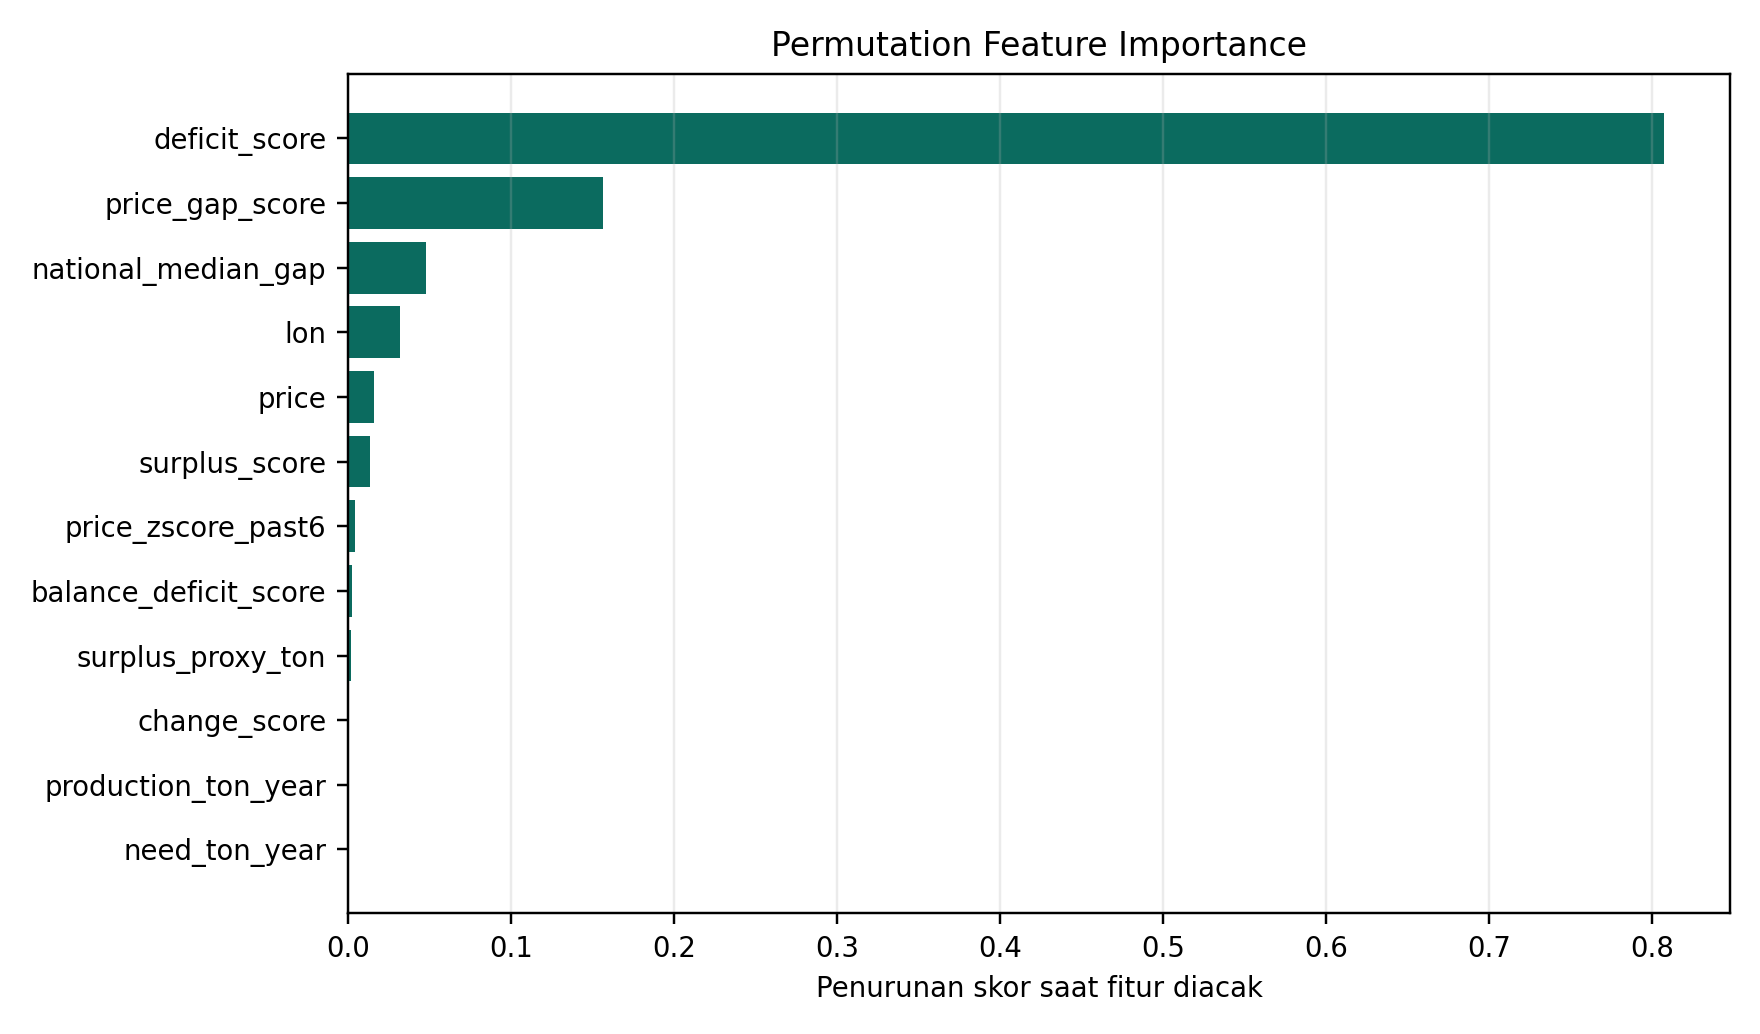
\includegraphics[width=0.48\columnwidth]{figures/feature_importance.png}
  \caption{Feature importance model prioritas.}
  \label{fig:feature_importance}
\end{figure}

\begin{figure}[H]
  \centering
  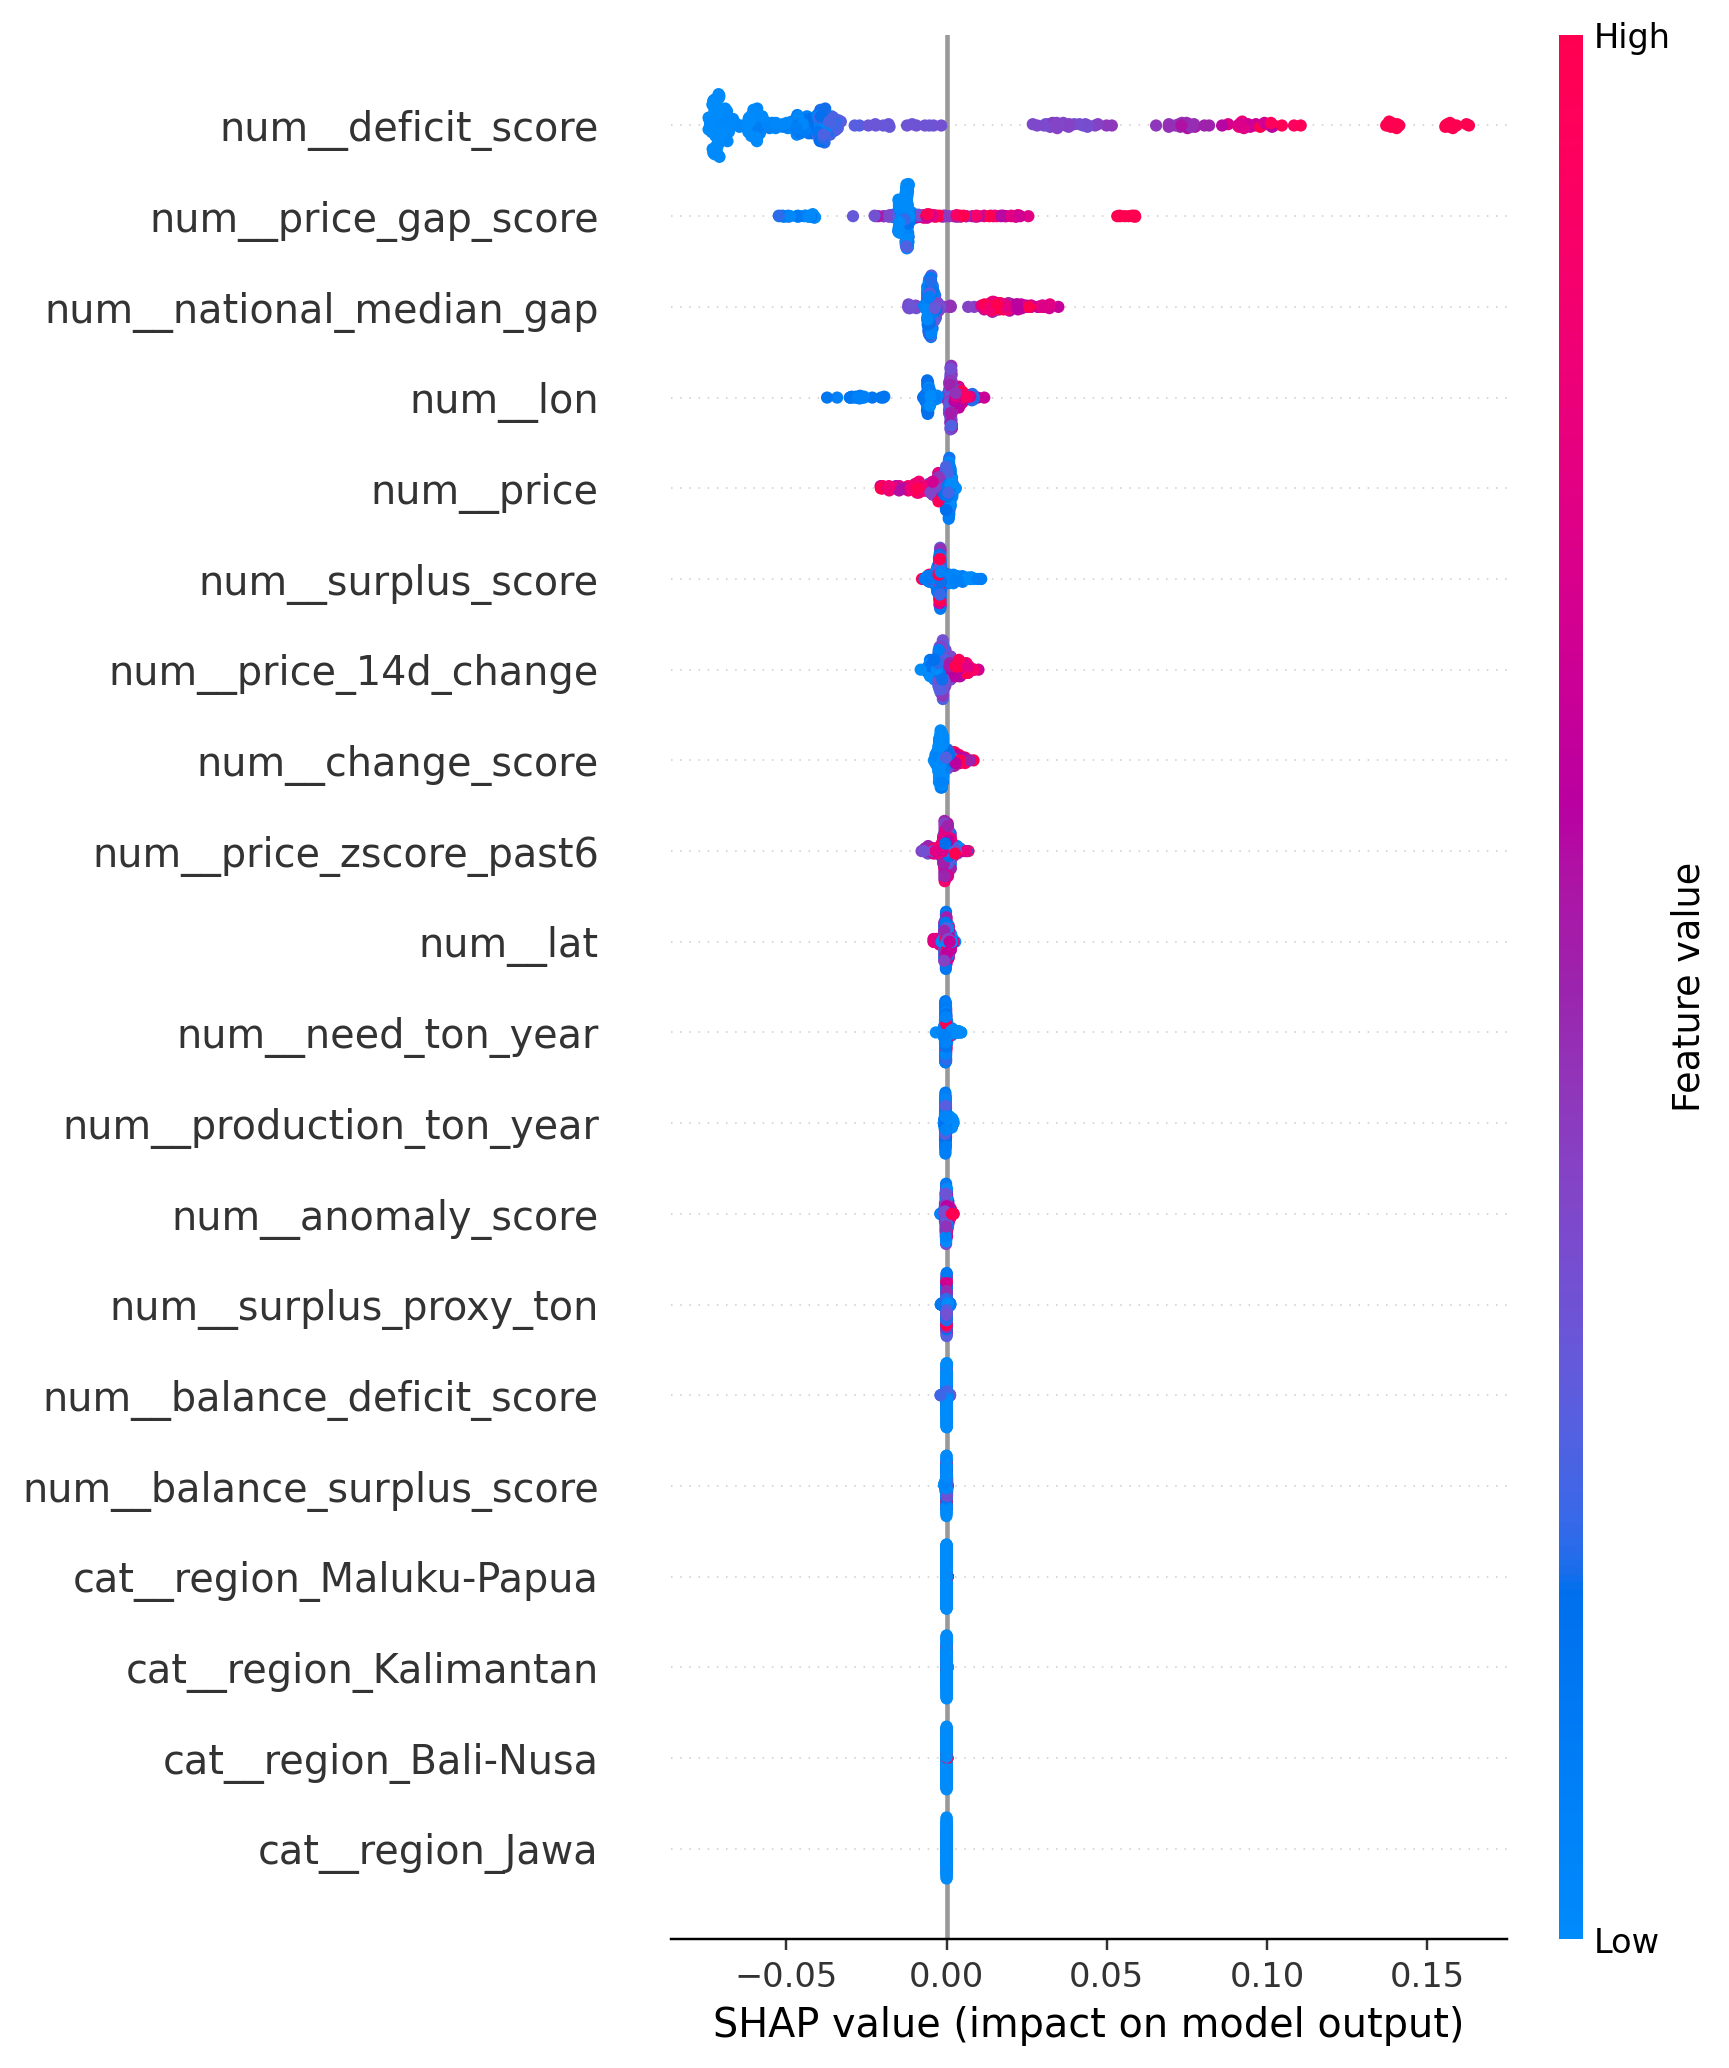
\includegraphics[width=0.48\columnwidth]{figures/shap_summary.png}
  \caption{SHAP summary plot -- kontribusi fitur terhadap output model.}
  \label{fig:shap_summary}
\end{figure}

\begin{table}[H]
  \footnotesize
  \caption{Top-5 provinsi dengan tingkat \textit{error} prediksi tertinggi.}
  \label{tab:error}
  \resizebox{\columnwidth}{!}{%
  \begin{tabular}{lrrr}
    \toprule
    Provinsi & Wilayah & MAE & RMSE \\
    \midrule
    Papua Pegunungan & Maluku-Papua & 0,202 & 0,224 \\
    Kalimantan Timur & Kalimantan & 0,117 & 0,124 \\
    Papua Tengah & Maluku-Papua & 0,105 & 0,118 \\
    DKI Jakarta & Jawa & 0,102 & 0,103 \\
    Maluku Utara & Maluku-Papua & 0,100 & 0,111 \\
    \bottomrule
  \end{tabular}%
  }
\end{table}




\section{Analisis Spasial dan Rekomendasi Aliran}
Peringkat prioritas daerah sasaran dan rekomendasi aliran (\textit{flow}) logistik beras dibangun menggunakan metode \textit{graph-based scoring} terpadu. Metode ini mengintegrasikan disparitas harga (\textit{price gap}), kapasitas surplus asal, tingkat defisit tujuan, serta penalti jarak spasial logistik. Model ini tidak ditujukan untuk menetapkan keputusan distribusi fisik mutlak, melainkan sebagai alat bantu prioritas pemantauan (\textit{review priority}) bagi pengambil kebijakan.

Hasil analisis spasial menunjukkan bahwa Papua Pegunungan menempati posisi provinsi tujuan utama pada 5 dari 6 rekomendasi aliran prioritas tertinggi. Tingginya prioritas wilayah ini disebabkan oleh harga eceran tertinggi nasional (Rp25.500/kg), defisit \textit{proxy} neraca beras tahunan sebesar 0,12 juta ton, serta skor anomali lonjakan harga mencapai 0,102. Sebaliknya, Sulawesi Selatan diposisikan sebagai provinsi asal redistribusi utama karena kapasitas surplus produksi lokalnya yang melimpah (2,31 juta ton) dengan tingkat harga eceran yang relatif rendah (Rp12.919/kg).

Hasil pemodelan menunjukkan dominasi provinsi dari region Maluku-Papua di peringkat prioritas, di mana 7 dari 10 provinsi sasaran utama beras berasal dari wilayah tersebut. Hal ini merefleksikan kondisi riil di lapangan, di mana seluruh provinsi di region Maluku-Papua secara historis mencatat defisit produksi pangan dan harga eceran beras di atas median nasional akibat jarak spasial yang sangat jauh dari sentra produksi beras nasional di Jawa dan Sulawesi.

Untuk rute lintas pulau jarak jauh seperti Sulawesi menuju Papua, kendala hambatan logistik direpresentasikan melalui penalti jarak \textit{distance\_penalty} sebesar -0,15 pada rumus \textit{scoring}. Dalam skenario ini, disparitas harga beras yang ekstrem (mencapai Rp12.581/kg) serta melimpahnya surplus di Sulawesi Selatan (2,31 juta ton) dapat mengompensasi penalti geografis tersebut, menempatkan koridor Sulawesi Selatan--Papua Pegunungan sebagai aliran dengan skor prioritas tertinggi (100,0).

\begin{table}[H]
  \footnotesize
  \caption{Rekomendasi aliran prioritas redistribusi beras.}
  \label{tab:flows}
  \resizebox{\columnwidth}{!}{%
  \begin{tabular}{lrrr}
    \toprule
    Peringkat & Provinsi Asal & Provinsi Tujuan & Skor Prioritas \\
    \midrule
    1 & Sulawesi Selatan & Papua Pegunungan & 100,0 \\
    2 & Jawa Timur & Papua Pegunungan & 95,54 \\
    3 & Jawa Tengah & Papua Pegunungan & 91,03 \\
    4 & Jawa Barat & Papua Pegunungan & 83,49 \\
    5 & Sumatera Selatan & Papua Pegunungan & 78,93 \\
    6 & Nusa Tenggara Barat & Papua Pegunungan & 76,72 \\
    \bottomrule
  \end{tabular}%
  }
\end{table}

Aliran Peringkat 1: Sulawesi Selatan menuju Papua Pegunungan memperoleh skor prioritas 100,0. Faktor pendukung utama meliputi: selisih harga beras sebesar Rp12.581/kg, kapasitas surplus produsen sebesar 2,31 juta ton, serta defisit lokal tujuan sebesar 0,12 juta ton. Rute logistik antarpulau ini memerlukan koordinasi distribusi lintas wilayah.

Aliran Peringkat 2: Jawa Timur menuju Papua Pegunungan memperoleh skor prioritas 95,54. Faktor pendukung utama meliputi: selisih harga beras sebesar Rp12.758/kg, kapasitas surplus produsen sebesar 2,14 juta ton, serta defisit lokal tujuan sebesar 0,12 juta ton.

Aliran Peringkat 3: Jawa Tengah menuju Papua Pegunungan memperoleh skor prioritas 91,03. Faktor pendukung utama meliputi: selisih harga beras sebesar Rp12.346/kg, kapasitas surplus produsen sebesar 1,97 juta ton, serta defisit lokal tujuan sebesar 0,12 juta ton.

\begin{figure}[H]
  \centering
  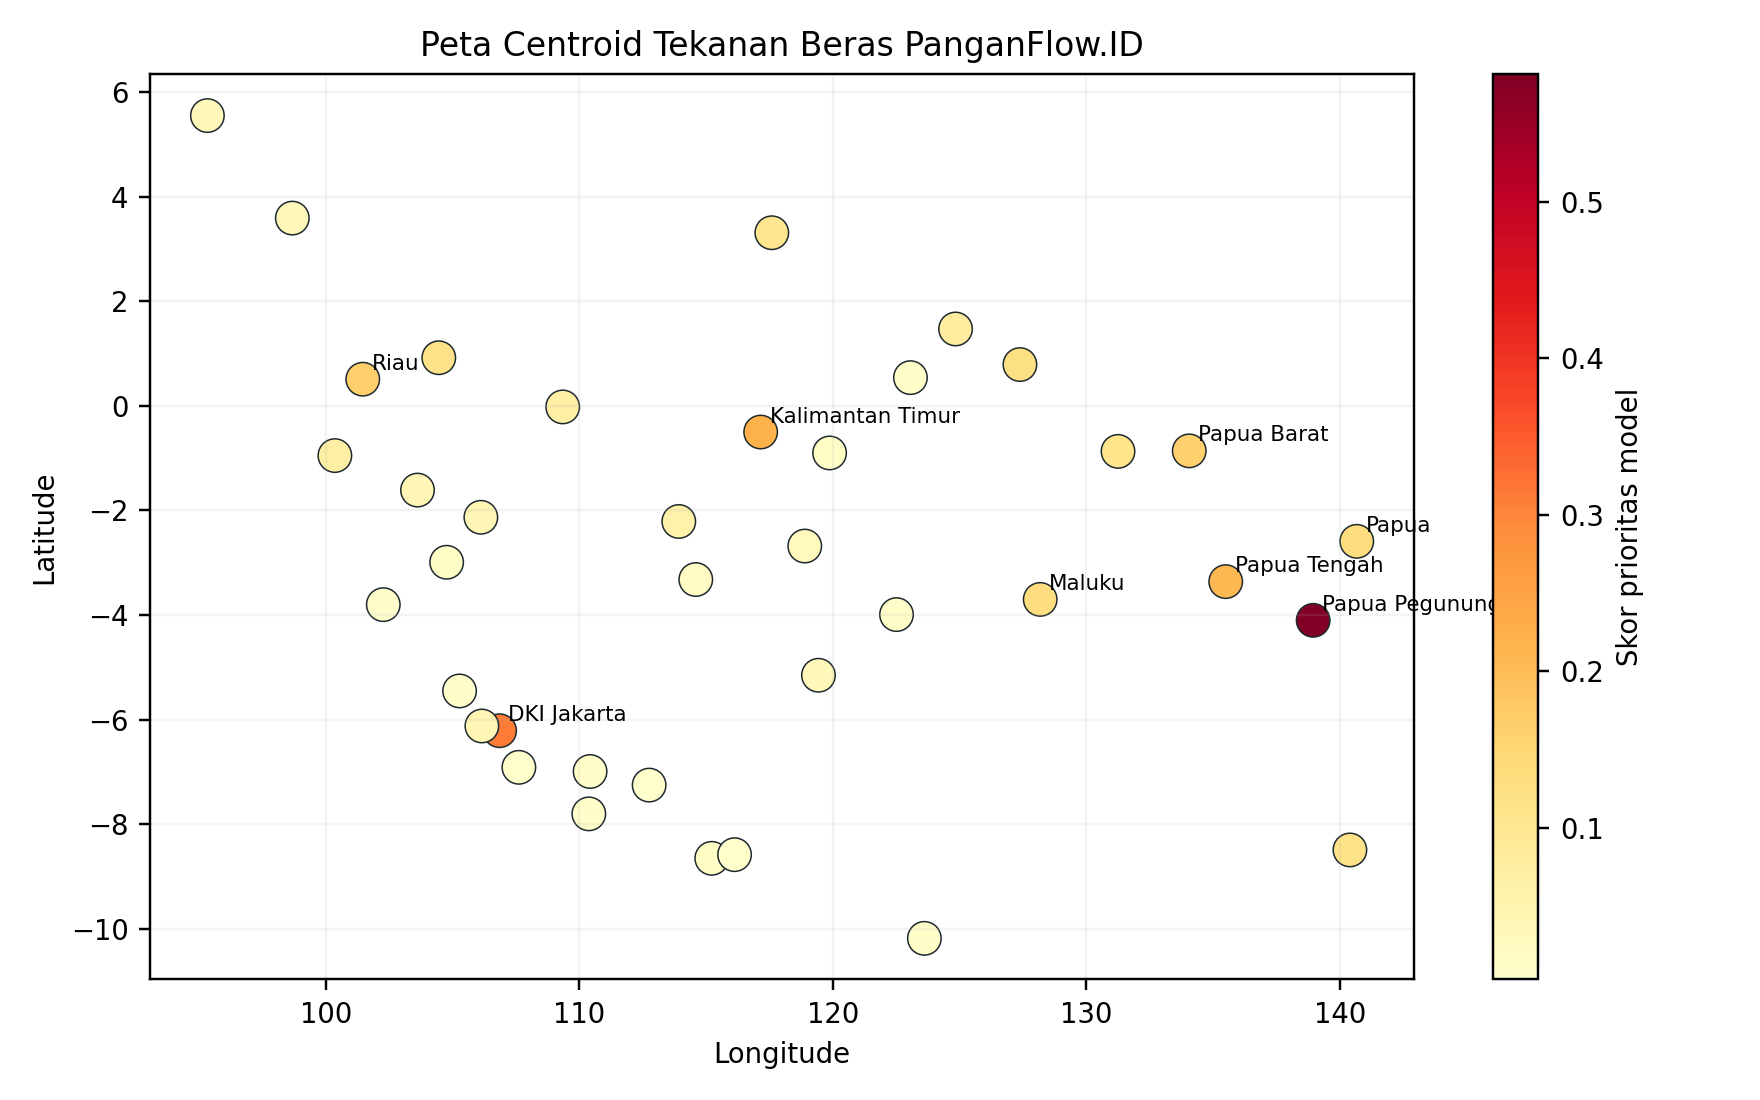
\includegraphics[width=0.48\columnwidth]{figures/pressure_centroid_map.png}
  \caption{Peta centroid tekanan beras nasional.}
  \label{fig:pressure_map}
\end{figure}

\begin{figure}[H]
  \centering
  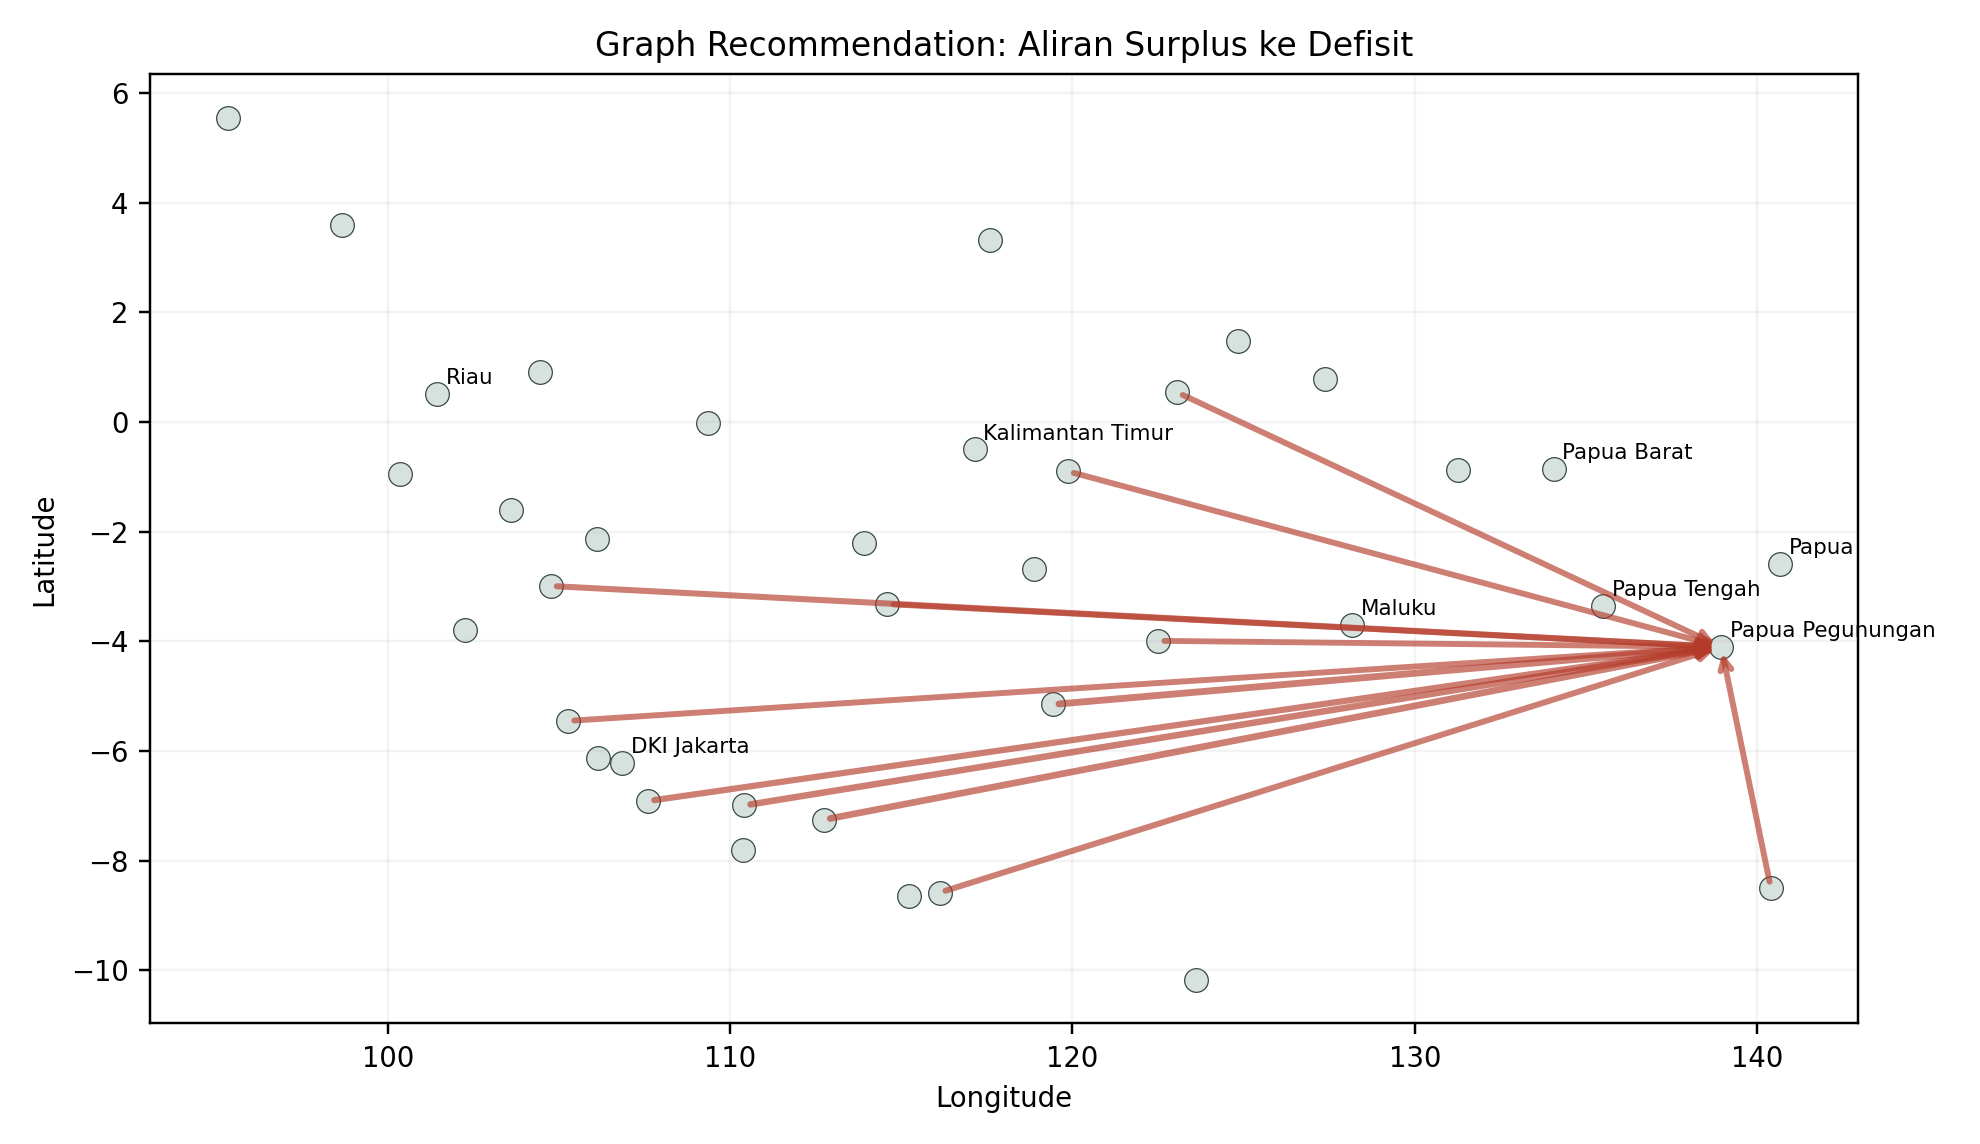
\includegraphics[width=0.48\columnwidth]{figures/flow_network.png}
  \caption{Visualisasi jaringan rekomendasi aliran antarprovinsi.}
  \label{fig:flow_network}
\end{figure}

\begin{figure}[H]
  \centering
  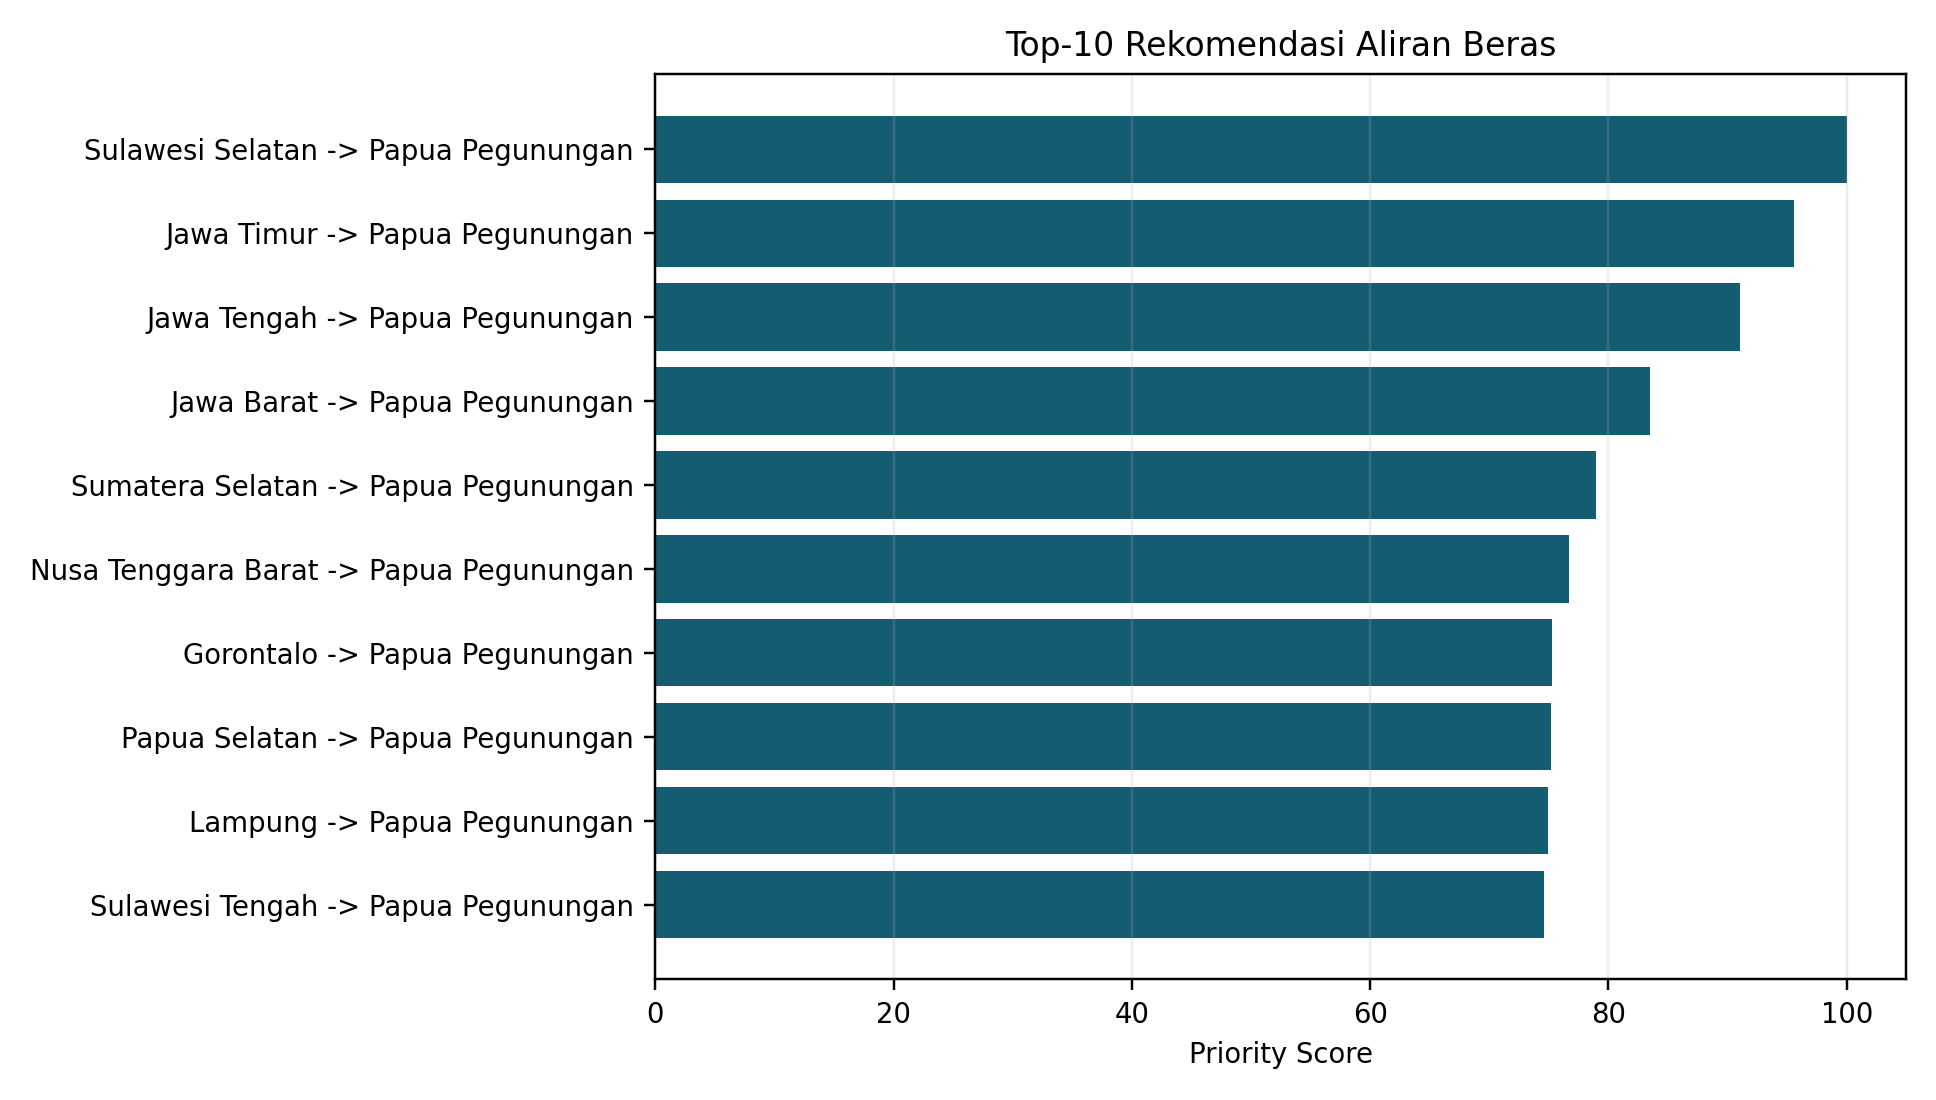
\includegraphics[width=0.48\columnwidth]{figures/top_flow_recommendations.png}
  \caption{Top-10 rekomendasi aliran beras nasional.}
  \label{fig:top_flows}
\end{figure}

\textbf{Implementasi Dashboard.} PanganFlow.ID dilengkapi dengan pratinjau sistem pemantauan interaktif (\textit{Watchboard}) berbasis Streamlit untuk memfasilitasi eksplorasi visual. Aplikasi dashboard ini terbagi dalam lima panel fungsional, yaitu: peta spasial tekanan pangan, daftar urutan prioritas wilayah, jaringan panah visualisasi rekomendasi \textit{flow}, rincian profil daerah, serta tab verifikasi kualitas dataset. Setiap rekomendasi aliran dilengkapi argumen penjelas secara otomatis (misalnya, ``selisih harga Rp12.581/kg; kapasitas surplus asal 2,31 juta ton'') untuk menunjang keterbacaan hasil model. Dashboard ini dapat dijalankan menggunakan perintah:
\texttt{python dashboard/app.py}.
\begin{figure}[H]
  \centering
  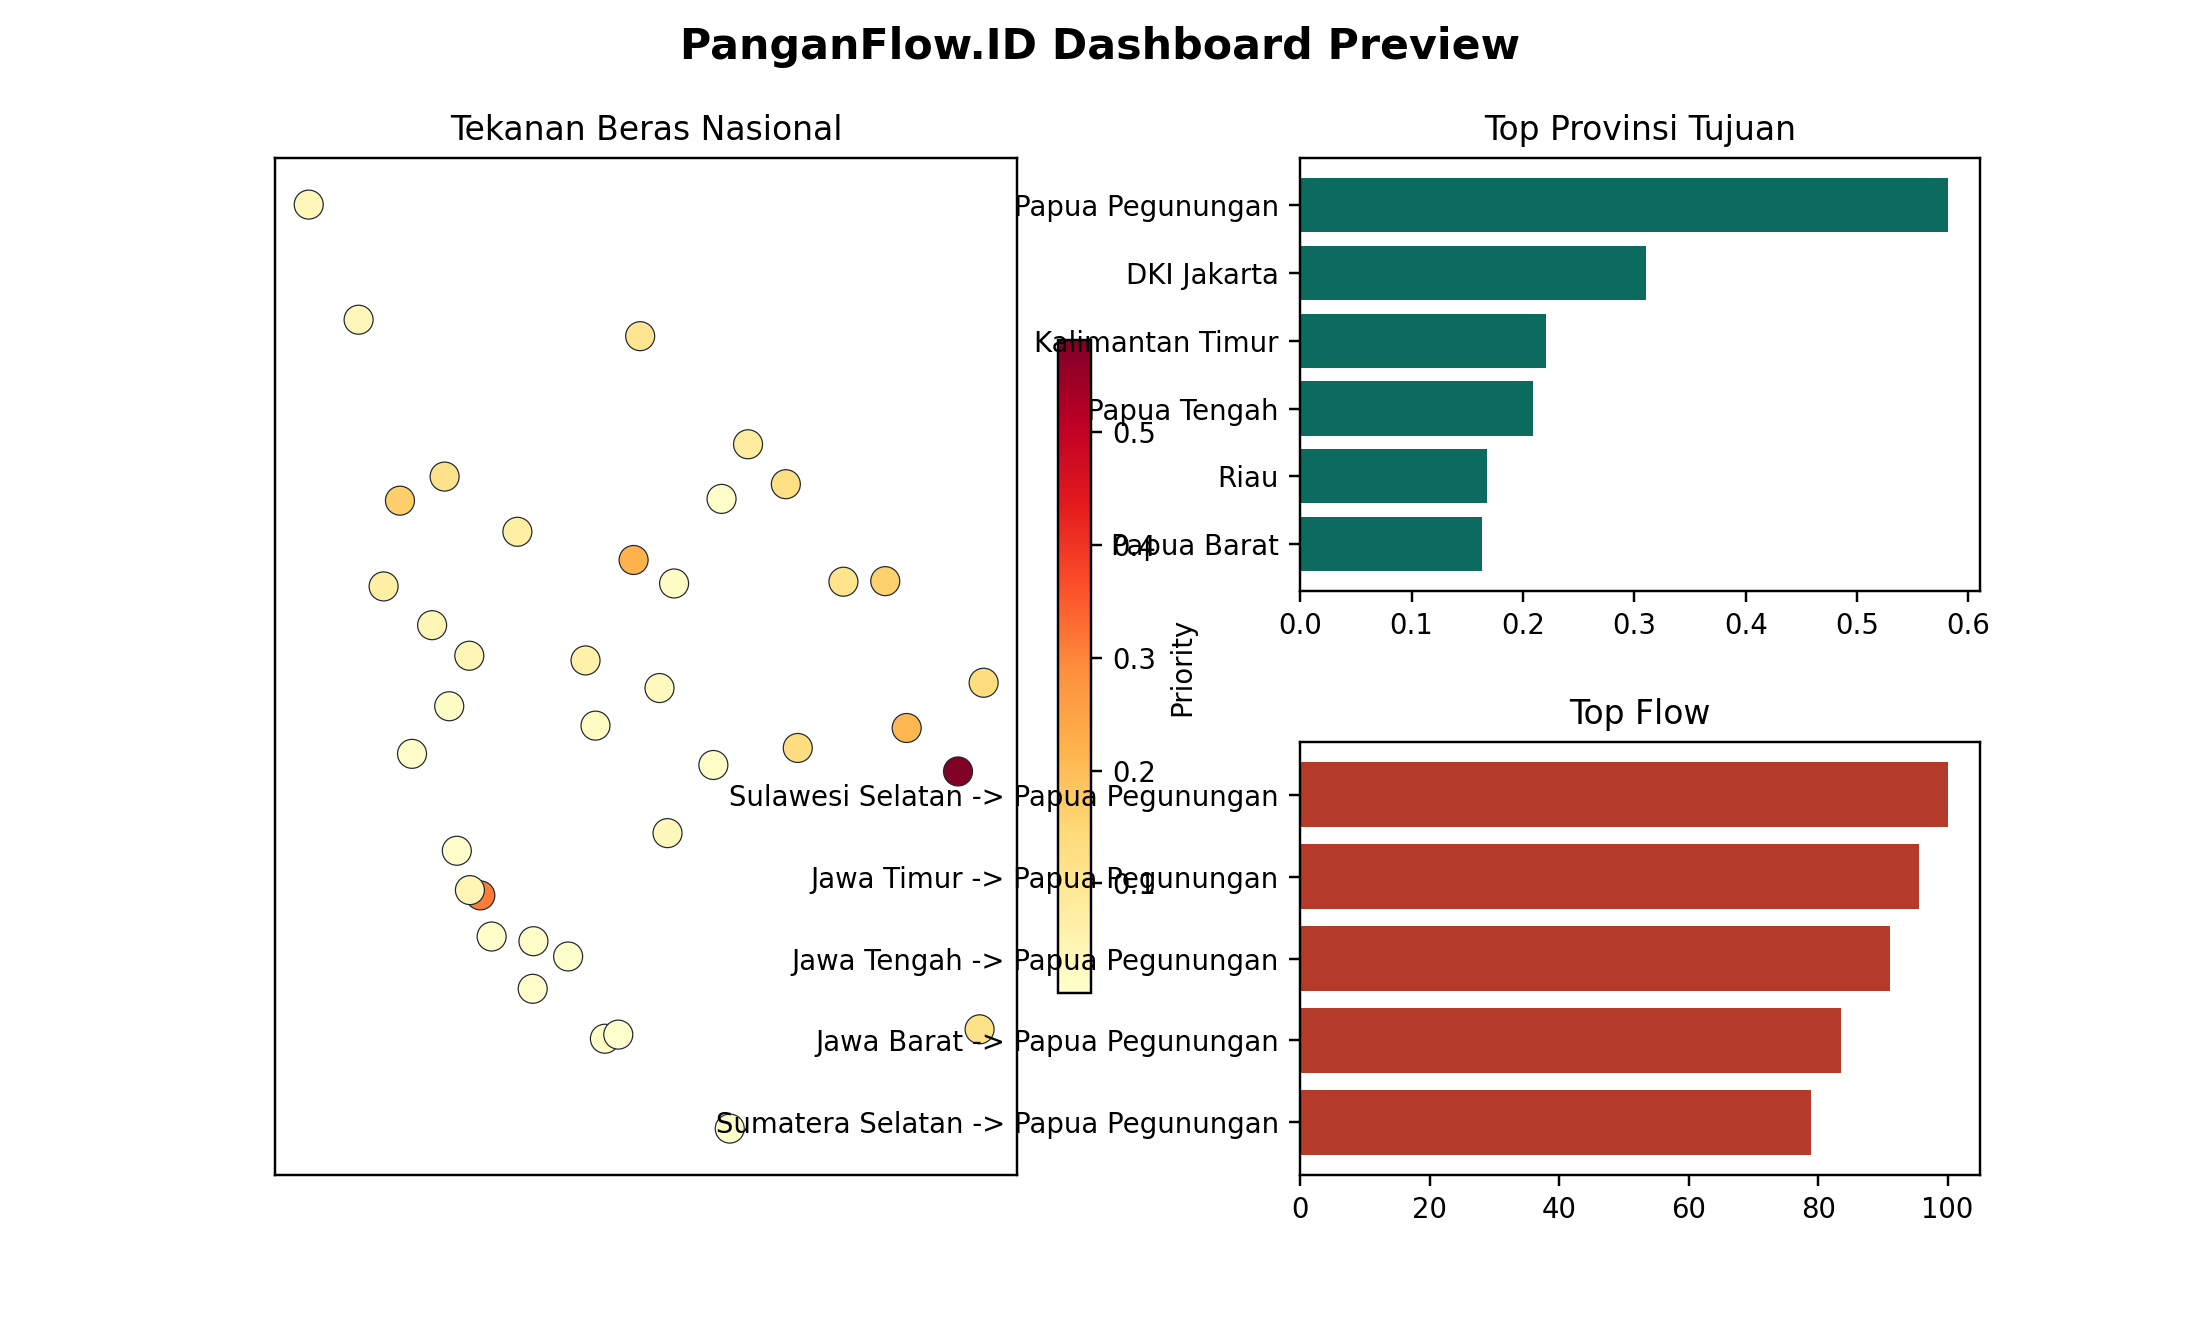
\includegraphics[width=0.45\columnwidth]{figures/dashboard_preview.png}
  \caption{Pratinjau antarmuka sistem PanganFlow.ID.}
  \label{fig:dashboard}
\end{figure}



\section{Clustering, Fairness, dan Studi Kasus}
Pemetaan tipologi spasial wilayah pangan dilakukan menggunakan algoritme \textit{K-Means clustering} untuk mengelompokkan 38 provinsi menjadi 4 klaster berdasarkan skor harga dan proxy neraca beras nasional (Tabel \ref{tab:clusters}). Hasil klasterisasi divisualisasikan dengan PCA pada Gambar \ref{fig:cluster_pca} yang memperlihatkan pemisahan klaster secara jelas.

\begin{table}[H]
  \caption{Ringkasan hasil pemetaan klaster tipologi provinsi.}
  \label{tab:clusters}
  \resizebox{\columnwidth}{!}{%
  \begin{tabular}{lrrr}
    \toprule
    Label Klaster & Jumlah Provinsi & Rerata Skor Defisit & Rerata Skor Surplus \\
    \midrule
    Defisit Kritis (Harga Sangat Tinggi) & 1 & 0,332 & 0,090 \\
    Defisit Moderat (Transisi/Rawan) & 12 & 0,149 & 0,232 \\
    Surplus Moderat (Relatif Aman) & 21 & 0,025 & 0,314 \\
    Surplus Melimpah (Sangat Stabil) & 4 & 0,003 & 0,879 \\
    \bottomrule
  \end{tabular}%
  }
\end{table}

\begin{figure}[H]
  \centering
  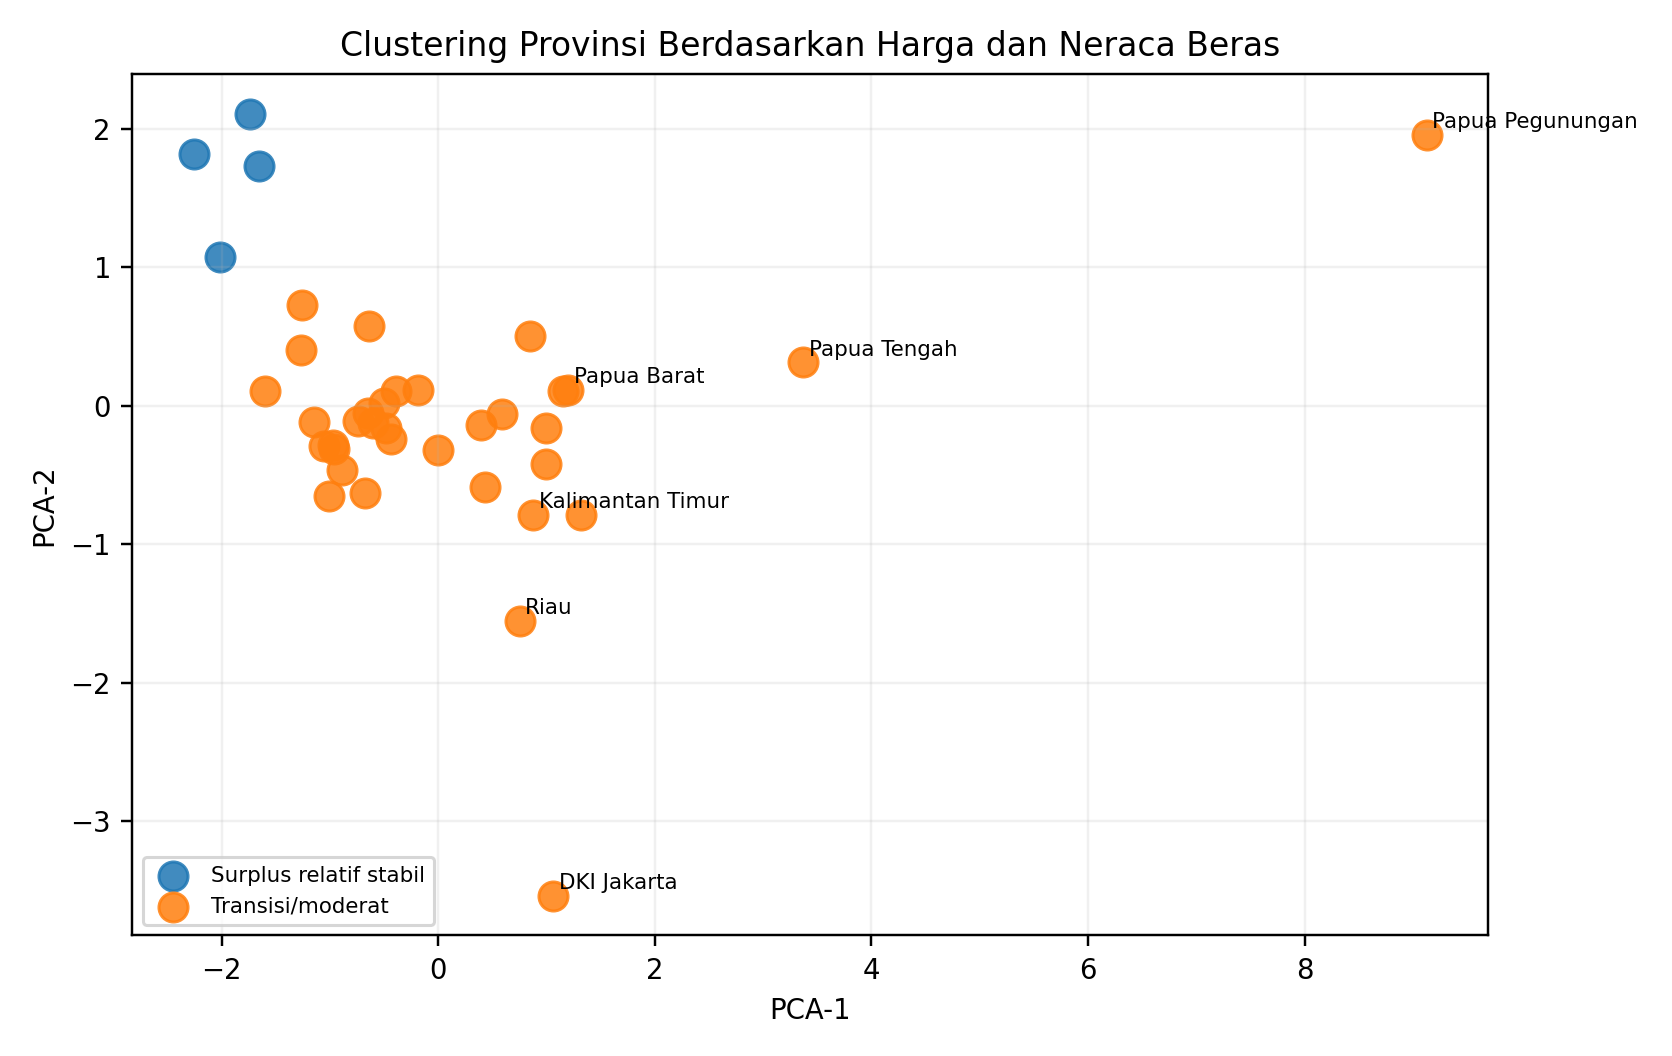
\includegraphics[width=0.48\columnwidth]{figures/cluster_pca.png}
  \caption{Visualisasi PCA klasterisasi provinsi.}
  \label{fig:cluster_pca}
\end{figure}

Evaluasi keadilan pemodelan (\textit{fairness analysis}) dilakukan melalui pemeriksaan subkelompok (\textit{subgroup analysis}) berbasis region (Tabel \ref{tab:fairness}) untuk mendeteksi potensi bias geografis. Hasil pengujian menunjukkan bahwa wilayah rentan seperti Maluku-Papua diakomodasi secara proporsional sesuai kondisi riil di lapangan.

\begin{table}[H]
  \footnotesize
  \caption{Pemeriksaan keadilan subkelompok (\textit{subgroup fairness}) berdasarkan region.}
  \label{tab:fairness}
  \resizebox{\columnwidth}{!}{%
  \begin{tabular}{lrrr}
    \toprule
    Wilayah & Jumlah Top-10 & Pangsa Top-10 & Rerata Skor Prioritas \\
    \midrule
    Maluku-Papua & 7 & 0,875 & 0,196 \\
    Kalimantan & 1 & 0,200 & 0,095 \\
    Jawa & 1 & 0,167 & 0,062 \\
    Sumatra & 1 & 0,100 & 0,053 \\
    Sulawesi & 0 & 0,000 & 0,029 \\
    Bali-Nusa & 0 & 0,000 & 0,009 \\
    \bottomrule
  \end{tabular}%
  }
\end{table}

\begin{table}[H]
  \footnotesize
  \caption{Studi kasus provinsi sasaran prioritas logistik.}
  \label{tab:cases}
  \resizebox{\columnwidth}{!}{%
  \begin{tabular}{llp{4.0cm}}
    \toprule
    Provinsi Tujuan & Rekomendasi Asal & Interpretasi Sinyal \\
    \midrule
    Papua Pegunungan & Sulawesi Selatan & Harga di atas median nasional; tren kenaikan positif; defisit \textit{proxy} neraca beras \\
    DKI Jakarta & Jawa Timur & Defisit \textit{proxy} neraca beras secara struktural \\
    Kalimantan Timur & Sulawesi Selatan & Harga di atas median nasional; defisit \textit{proxy} neraca beras \\
    Papua Tengah & Sulawesi Selatan & Harga di atas median nasional; tren kenaikan positif; defisit \textit{proxy} neraca beras \\
    \bottomrule
  \end{tabular}%
  }
\end{table}

Pemeriksaan stabilitas model melalui perturbasi acak pada skor input (\textit{stability check}) menghasilkan rata-rata \textit{overlap} peringkat Top-10 sebesar 0,863. Hasil ini menunjukkan stabilitas peringkat PanganFlow.ID terhadap fluktuasi data minor di lapangan.



\section{Kesimpulan}
Penelitian ini menunjukkan bahwa integrasi data multi-sumber (harga Bapanas, produksi-konsumsi BPS, spasial Haversine) melalui analisis \textit{data mining} spatio-temporal dapat menghasilkan rekomendasi aliran pangan guna mendukung kemandirian pangan nasional. Model hibrida PanganFlow mencapai performa NDCG@K sebesar 0,937, mengungguli baseline pembanding (\textit{random}, \textit{price-gap}, \textit{deficit}, dan \textit{weighted index}).

Studi ablasi menunjukkan bahwa kelompok fitur neraca pangan (\textit{balance}) merupakan kontributor terbesar terhadap performa model, di mana ketiadaannya memicu penurunan performa NDCG@K dari 0,905 menjadi 0,880 (reduksi sebesar 2,8\%). Sebaliknya, fitur spasial geografis memberikan kontribusi marginal terkecil (tanpa spasial: NDCG@K=0,912) karena interaksi jarak logistik spasial sebagian besar telah terwadahi oleh variabel pengelompokan wilayah geografis (\textit{region grouping}).

Analisis \textit{error} spasial menunjukkan region Maluku-Papua memiliki rata-rata MAE tertinggi (0,098), dengan Papua Pegunungan sebagai wilayah dengan kompleksitas prediksi terbesar (MAE=0,202). Hal ini selaras dengan kondisi riil volatilitas harga ekstrem dan tantangan rantai pasok logistik di Indonesia bagian timur. Uji stabilitas peringkat dengan \textit{bootstrap} 120 \textit{run} menghasilkan rata-rata tingkat tumpang tindih (\textit{overlap}) Top-10 sebesar 0,863, menunjukkan tingkat ketahanan peringkat model.

Pengembangan riset selanjutnya dapat ditingkatkan melalui integrasi indikator dinamis tambahan seperti stok riil gudang bulog bulanan, kalender musim tanam-panen regional, serta indikator hambatan logistik pelabuhan laut guna memperkaya akurasi rute aliran logistik pangan aktual nasional.

Keterbatasan penelitian ini mencakup beberapa aspek utama: (1) estimasi neraca menggunakan \textit{proxy} populasi tahunan sehingga belum menangkap fluktuasi stok fisik riil bulanan; (2) data harga Bapanas bulanan berfokus pada kestabilan tren nasional namun kurang sensitif dibanding data harian; (3) jarak spasial dihitung berdasarkan \textit{Haversine centroid} wilayah, sehingga belum menggambarkan rute pelayaran dan kapasitas pelabuhan riil; dan (4) model mempelajari prioritas intervensi berbasis data historis, bukan mencerminkan keputusan kebijakan politik operasional langsung pemerintah.



\begin{thebibliography}{99}
  \bibitem{1} E. Sediyono and D. Hartomo, ``An Integrated Framework for Multi-Commodity Agricultural Price Forecasting and Anomaly Detection,'' Semantic Scholar, 2025.
  \bibitem{2} ``Temporal and Semantic Fusion with Agentic AI for Commodity Price Shock Forecasting,'' \href{https://arxiv.org/abs/2508.06497}{arXiv:2508.06497}, 2025.
  \bibitem{3} ``Perbandingan Kinerja LSTM, Random Forest, dan SVR untuk Prediksi Harga Beras,'' JURIKOM, 2024.
  \bibitem{4} ``Komparasi Model ARIMA, Regresi Linear, Random Forest, dan LSTM untuk Prediksi Harga Beras,'' JIT Nurulfikri, 2024.
  \bibitem{5} ``Rice Price Prediction in East Java Based on Weather Using LSTM,'' JAIC Polibatam, 2025.
  \bibitem{6} ``Performance Evaluation of Ensemble Learning Stacking in Rice Price Prediction,'' \href{https://doi.org/10.1109/10957374}{IEEE, 2024}.
  \bibitem{7} ``Advanced Deep Learning and Hybrid Models for Forecasting Rice Production in Indonesia,'' ITS Scholar, 2024.
  \bibitem{8} ``Forecasting and Spatial Distribution Analysis of Cold Chain Logistics,'' \href{https://doi.org/10.1007/s10668-025-06969-9}{Springer, 2025}.
  \bibitem{9} ``Crop Redistribution Increases Regional Production While Reducing Resource Use,'' MDPI Agronomy, 15(9), 2148, 2025.
  \bibitem{10} ``Spatial Equilibrium Model-Based Optimization for Inter-Regional Grain Trade,'' Water Supply, 22(5), 5393, \href{https://iwaponline.com/ws/article/22/5/5393}{2022}.
  \bibitem{11} L. Breiman, ``Random Forests,'' Machine Learning, 45(1), 5--32, \href{https://doi.org/10.1023/A:1010933404324}{2001}.
  \bibitem{12} F. T. Liu, K. M. Ting, and Z. H. Zhou, ``Isolation Forest,'' \href{https://doi.org/10.1109/ICDM.2008.17}{ICDM, 2008}.
  \bibitem{13} J. MacQueen, ``Some Methods for Classification and Analysis of Multivariate Observations,'' \href{https://projecteuclid.org/euclid.bsmsp/1200512992}{Berkeley Symposium, 1967}.
  \bibitem{14} Bank Indonesia, ``Pusat Informasi Harga Pangan Strategis Nasional,'' \href{https://www.bi.go.id/hargapangan}{bi.go.id/hargapangan}.
  \bibitem{15} Badan Pangan Nasional, ``Rata-rata Harga Pangan Bulanan Tingkat Konsumen Provinsi,'' \href{https://satudata.badanpangan.go.id}{satudata.badanpangan.go.id}.
  \bibitem{16} Badan Pusat Statistik, ``Produksi Padi dan Beras Menurut Provinsi,'' \href{https://www.bps.go.id}{bps.go.id}, 2024.
  \bibitem{17} Badan Pusat Statistik, ``Pengeluaran untuk Konsumsi Penduduk Indonesia per Provinsi,'' \href{https://www.bps.go.id}{bps.go.id}, 2024.
\end{thebibliography}


\end{document}
